% Created 2018-10-18 jue 15:29
% Intended LaTeX compiler: pdflatex
\documentclass[xcolor={usenames,svgnames,dvipsnames}]{beamer}
\usepackage[utf8]{inputenc}
\usepackage[T1]{fontenc}
\usepackage{graphicx}
\usepackage{grffile}
\usepackage{longtable}
\usepackage{wrapfig}
\usepackage{rotating}
\usepackage[normalem]{ulem}
\usepackage{amsmath}
\usepackage{textcomp}
\usepackage{amssymb}
\usepackage{capt-of}
\usepackage{hyperref}
\usepackage{color}
\usepackage{listings}
\usepackage{mathpazo}
\usepackage{gensymb}
\usepackage{amsmath}
\usepackage{chemarr}%flechas para reacciones químicas (SFER.tex)
\bibliographystyle{plain}
\AtBeginSubsection[]{\begin{frame}[plain]\tableofcontents[currentsubsection,sectionstyle=show/shaded,subsectionstyle=show/shaded/hide]\end{frame}}
\AtBeginSection[]{\begin{frame}[plain]\tableofcontents[currentsection,hideallsubsections]\end{frame}}
\usepackage[emulate=units]{siunitx}
\sisetup{fraction=nice, decimalsymbol=comma, retain-unity-mantissa = false}
\newunit{\wattpeak}{Wp}
\newunit{\watthour}{Wh}
\newunit{\amperehour}{Ah}
\hypersetup{colorlinks=true, linkcolor=Blue, urlcolor=Blue}
\renewcommand{\thefootnote}{\fnsymbol{footnote}}
\beamertemplatenavigationsymbolsempty
\setbeamertemplate{footline}[frame number]
\setbeamercolor{alerted text}{fg=blue!50!black} \setbeamerfont{alerted text}{series=\bfseries}
\usetheme[hideothersubsections]{Goettingen}
\usecolortheme{rose}
\usefonttheme{serif}
\author{Oscar Perpiñán Lamigueiro \\ \url{http://oscarperpinan.github.io}}
\date{}
\title{Electrotecnia}
\hypersetup{
 pdfauthor={Oscar Perpiñán Lamigueiro \\ \url{http://oscarperpinan.github.io}},
 pdftitle={Electrotecnia},
 pdfkeywords={},
 pdfsubject={},
 pdfcreator={Emacs 25.2.2 (Org mode 9.1.13)}, 
 pdflang={Spanish}}
\begin{document}

\maketitle

\section{Conceptos preliminares}
\label{sec:org97a0282}


\subsection{Definiciones}
\label{sec:orgeb12edf}


\begin{frame}[label={sec:orga4c14f4}]{Sistema de suministro eléctrico}
Un \alert{sistema de suministro eléctrico} tiene como objetivo \alert{producir,
transportar y distribuir energía eléctrica} a los lugares de consumo,
con el mínimo coste posible en condiciones de \alert{fiabilidad, calidad y
seguridad}.
\end{frame}

\begin{frame}[label={sec:orge23dda1}]{Componentes del Sistema de Suministro Eléctrico}
\begin{center}
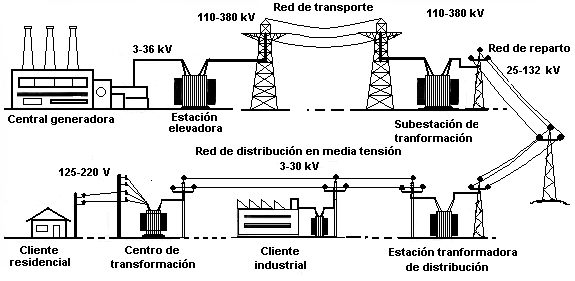
\includegraphics[width=.9\linewidth]{../figs/Redelectrica2.png}
\end{center}

\begin{itemize}
\item Generadores

\item Redes de transporte

\item Redes de distribución

\item Equipos de acondicionamiento, transformación y protección (y en
algunos casos, almacenamiento)

\item Puntos de consumo
\end{itemize}
\end{frame}

\begin{frame}[label={sec:org8a0378b}]{Electricidad}
\begin{itemize}
\item La electricidad es un fenómeno físico asociado al \alert{movimiento de las
cargas eléctricas}.

\item El aprovechamiento de la electricidad consiste en generar y canalizar
el movimiento de las cargas eléctricas.

\item El movimiento de las cargas eléctricas es la \alert{corriente eléctrica}.
Este movimiento se realiza mediante un trabajo, cuantificado por el
\alert{potencial}.
\end{itemize}
\end{frame}

\begin{frame}[label={sec:orgd0188bd}]{Intensidad de Corriente eléctrica}
\begin{itemize}
\item \alert{Variación de la carga con el tiempo en la sección transversal de un
conductor} $$i(t)=\frac{dq(t)}{dt}$$

\item Movimiento de electrones libres. Sin embargo, por convenio su sentido
es positivo para el movimiento de las cargas positivas.
\end{itemize}
\end{frame}

\begin{frame}[label={sec:org9c2c4f8}]{Intensidad de Corriente Eléctrica}
\begin{itemize}
\item \alert{Principio de conservación de la carga}: las lineas de corriente son
cerradas (o solenoidales)

\begin{itemize}
\item Primera ley de Kirchhoff : la suma de las corrientes que llegan a
un nudo es igual a la suma de las que salen.
\end{itemize}
\end{itemize}
\end{frame}

\begin{frame}[label={sec:orgb518658}]{Tensión. Diferencia de potencial}
\begin{itemize}
\item \alert{Trabajo realizado al mover una carga unidad entre dos puntos}.
\end{itemize}

$$v=\frac{dW_{e}}{dq}$$

\begin{itemize}
\item Si entre dos puntos A y B existe una diferencia de potencial, podemos
escribir: $$\begin{aligned}
         v_{AB} & = & v_{A}-v_{B}\\
         v_{AB} & = & -v_{BA}
       \end{aligned}$$
\end{itemize}
\end{frame}

\begin{frame}[label={sec:orgf6017ec}]{Tensión Eléctrica}
\begin{itemize}
\item \alert{Principio de conservación de la energía}: la energía producida por
un generador se consume por los receptores del circuito para producir
trabajo (mecánico, químico, etc.) o calor.

\begin{itemize}
\item Segunda ley de Kirchhoff: la suma (con signo) de las tensiones a
lo largo de un camino cerrado (circuito) es cero
\end{itemize}
\end{itemize}
\end{frame}


\begin{frame}[label={sec:org66869f1}]{Potencia eléctrica}
\begin{itemize}
\item Trabajo realizado por unidad de tiempo
\end{itemize}
\[
p(t)=\frac{dW_{e}}{dt}=v(t)\cdot\frac{dq(t)}{dt}=v(t)\cdot i(t)
\]

\begin{itemize}
\item Un elemento del circuito absorbe (\emph{receptor}) o entrega
(\emph{generador}) potencia según el sentido de tensión y corriente en
sus terminales. Ejemplo: en el dipolo de la figura se absorbe
potencia (\(p(t)>0\))
\end{itemize}
\begin{center}
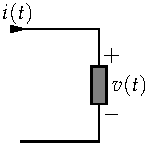
\includegraphics[height=0.5\textheight]{../figs/ReceptorPasivo.pdf}
\end{center}
\end{frame}

\begin{frame}[label={sec:org14f8314}]{Potencia y Energía}
\begin{description}
\item[{Energía}] es la capacidad para realizar un trabajo.

Unidades Wh, kWh

1 kWh = 3.6 MJ

\item[{Potencia}] es la cantidad de trabajo efectuado \emph{por unidad de
tiempo}.

Unidades W, kW
\end{description}
\end{frame}

\begin{frame}[label={sec:orgf471142}]{Eficiencia y Rendimiento}
\begin{description}
\item[{Eficiencia}] de un proceso es la relación entre la \emph{potencia} de
salida y la \emph{potencia} de entrada a ese proceso.

\item[{Rendimiento}] de un proceso es la relación entre la \emph{energía} de
salida y la \emph{energía} de entrada a ese proceso.
\end{description}
\end{frame}

\subsection{Elementos Lineales}
\label{sec:org04424e2}

\begin{frame}[label={sec:org871fe8b}]{Generadores}
\begin{itemize}
\item \alert{Generador de tensión}: su tensión es independiente de la corriente
(la corriente la fija el circuito)

\begin{itemize}
\item Batería electroquímica

\item Inversor de electrificación rural a su salida
\end{itemize}
\end{itemize}
\begin{center}
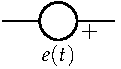
\includegraphics[height=0.2\textheight]{../figs/GeneradorTension.pdf}
\end{center}

\begin{itemize}
\item \alert{Generador de corriente}: su corriente es independiente de la tensión
(la tensión la fija el circuito)

\begin{itemize}
\item Inversor de conexión a red a su salida
\end{itemize}
\end{itemize}
\begin{center}
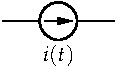
\includegraphics[height=0.2\textheight]{../figs/GeneradorCorriente.pdf}
\end{center}
\end{frame}

\begin{frame}[label={sec:org66f2a67}]{Resistencia}
\begin{center}
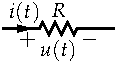
\includegraphics[height=0.2\textheight]{../figs/Resistencia.pdf}
\end{center}


\begin{itemize}
\item \alert{Produce una caída de tensión entre sus terminales directamente
proporcional a la corriente que lo atraviesa}.

\item La constante de proporcionalidad es el valor de la resistencia:
\(V=R\cdot I\)

\item Su valor depende de resistividad del material, de la sección y de la
longitud: \(R=\rho\cdot\frac{L}{S}\)
\end{itemize}
\end{frame}

\begin{frame}[label={sec:org953ba97}]{Resistencia}
\begin{center}
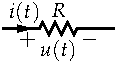
\includegraphics[height=0.2\textheight]{../figs/Resistencia.pdf}
\end{center}


\begin{itemize}
\item Disipa energía eléctrica produciendo \alert{calor}: \(p(t)=R\cdot i^{2}(t)\)

\item Cortocircuito: resistencia nula (tensión nula)

\item Circuito abierto: resistencia infinita (corriente nula).
\end{itemize}
\end{frame}


\begin{frame}[label={sec:orgd907ea3}]{Bobina o inductancia}
\begin{center}
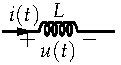
\includegraphics[height=0.2\textheight]{../figs/Bobina.pdf}
\end{center}


\begin{itemize}
\item Cuando una corriente oscilante atraviesa un conductor arrollado se
produce una \alert{tensión inducida que se opone a esta corriente} (ley de
Faraday y Lenz)

\item La constante que liga la tensión en sus terminales con el cambio de
la corriente es el valor de la inductancia
$$v(t)=L\cdot\frac{di(t)}{dt}$$
\end{itemize}
\end{frame}

\begin{frame}[label={sec:org94d8991}]{Bobina o inductancia}
\begin{center}
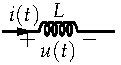
\includegraphics[height=0.2\textheight]{../figs/Bobina.pdf}
\end{center}


\begin{itemize}
\item Almacena \alert{energía magnética}.

\item La bobina \alert{retrasa los cambios de la corriente} respecto de la
tensión.

\item En circuitos de corriente continua es un cortocircuito.
\end{itemize}
\end{frame}

\begin{frame}[label={sec:org990e2b5}]{Condensador}
\begin{center}
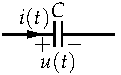
\includegraphics[height=0.2\textheight]{../figs/Condensador.pdf}
\end{center}

\begin{itemize}
\item Cuando se establece una tensión entre dos placas metálicas separadas
por una capa dieléctrica, se produce una \alert{separación de cargas que se
acumulan en cada placa}, con signos contrarios.

\item La constante de proporcionalidad entre la carga acumulada y la
tensión entre las placas es la capacidad $$C=\frac{Q}{V_{AB}}$$
\end{itemize}
\end{frame}


\begin{frame}[label={sec:org2f6d459}]{Condensador}
\begin{center}
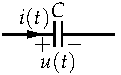
\includegraphics[height=0.2\textheight]{../figs/Condensador.pdf}
\end{center}

\begin{itemize}
\item En el proceso de carga se produce una corriente eléctrica entre las
dos placas $$i(t)=\frac{dq(t)}{d(t)}=C\frac{dv(t)}{dt}$$

\item Almacena \alert{energía eléctrica}

\item \alert{Retrasa las variaciones de la tensión respecto de la corriente}

\item En un circuito de corriente continua cuando el condensador está
cargado se comporta como un circuito abierto.
\end{itemize}
\end{frame}

\subsection{Elementos No Lineales}
\label{sec:org4044d33}

\begin{frame}[label={sec:org35b856a}]{Diodo}
\begin{center}
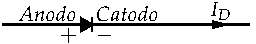
\includegraphics[height=0.15\textheight]{../figs/Diodo.pdf}
\end{center}

\begin{itemize}
\item Un diodo es un dispositivo electrónico que permite el paso de
corriente a través de él a partir de una tensión de polarización.

\item Cuando no conduce se comporta (idealmente) como un circuito abierto.
Cuando conduce se comporta (idealmente) como un cortocircuito.
\end{itemize}
\end{frame}

\begin{frame}[label={sec:org81c29e1}]{Diodo}
\begin{center}
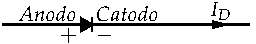
\includegraphics[height=0.15\textheight]{../figs/Diodo.pdf}
\end{center}

\begin{itemize}
\item Por tanto, puede ser utilizado como

\begin{itemize}
\item \alert{Elemento de bloqueo} (evitar que circule corriente por una parte
del circuito en ciertas condiciones)

\item \alert{Elemento de protección} (obligar a que la corriente circule por
él, evitando que circule por otra rama paralela).
\end{itemize}
\end{itemize}
\end{frame}

\begin{frame}[label={sec:orgd7978ec}]{Transistor}
\begin{center}
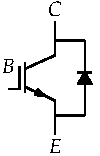
\includegraphics[height=0.3\textheight]{../figs/Transistor.pdf}
\end{center}

\begin{itemize}
\item Un transistor es un dispositivo electrónico con tres terminales que
permite el paso de corriente entre dos de sus terminales cuando en el
tercer terminal está polarizado adecuadamente.

\item Cuando no conduce se comporta (idealmente) como un circuito abierto.

\item Cuando conduce se comporta (idealmente) como un cortocircuito.
\end{itemize}
\end{frame}


\begin{frame}[label={sec:org5d0c28f}]{Transistor}
\begin{center}
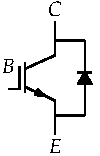
\includegraphics[height=0.3\textheight]{../figs/Transistor.pdf}
\end{center}

Por tanto, puede ser utilizado como:

\begin{itemize}
\item \alert{Elemento de conmutación} (dirigir la circulación de corriente entre
dos terminales controlando la señal en el tercer terminal)

\item \alert{Elemento de amplificación} (la señal entregada en el terminal de
control es reproducida en la salida con mayor amplitud)
\end{itemize}
\end{frame}

\subsection{Asociación de elementos pasivos}
\label{sec:orgf39b710}

\begin{frame}[label={sec:orgdffc688}]{Conexión en serie}
\begin{block}{Misma corriente por todos los elementos: la tensión se reparte}
\(R_{s}=\sum_{i}R_{i}\)

\(L_{s}=\sum_{i}L_{i}\)

\(\frac{1}{C_{s}}=\sum_{i}\frac{1}{C_{i}}\)
\begin{center}
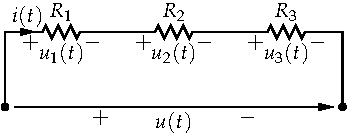
\includegraphics[height=0.3\textheight]{../figs/AsociacionSerie.pdf}
\end{center}
\end{block}
\end{frame}

\begin{frame}[label={sec:org523c0e8}]{Conexión en paralelo}
\begin{block}{Misma tensión aplicada a todos los elementos: la corriente se reparte}
\(\frac{1}{R_{p}}=\sum_{i}\frac{1}{R_{i}}\)

\(\frac{1}{L_{p}}=\sum_{i}\frac{1}{L_{i}}\)

\(C_{p}=\sum_{i}C_{i}\)
\begin{center}
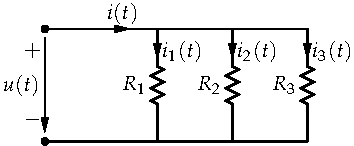
\includegraphics[height=0.3\textheight]{../figs/AsociacionParalelo.pdf}
\end{center}
\end{block}
\end{frame}

\section{Corriente alterna sinusoidal}
\label{sec:org0c07afd}

\subsection{Conceptos Fundamentales}
\label{sec:org397ab4d}

\begin{frame}[label={sec:org681cc76}]{Pulsación - Frecuencia - Fase}
\[
y(t)=Y_{o}\cdot\cos(\omega\cdot t+\varphi)
\]

\begin{itemize}
\item \(Y_{o}\) valor máximo de la onda.

\item \(\omega=\frac{2\cdot\pi}{T}\): pulsación (radianes/segundo)

\item T: periodo de la onda (segundos)

\item \(f=\frac{\omega}{2\cdot\pi}=\frac{1}{T}\): frecuencia (Hz)

\item \(\varphi\): fase (radianes o grados)

\begin{itemize}
\item Es el argumento de la onda para t=0

\item Tomando una onda como referencia, si la fase es 0º, se dice que
están en fase con la onda de referencia.

\item Ídem, si la fase es 90º, se dice que están en cuadratura.

\item Ídem, si la fase es positiva, se dice que la onda adelanta
respecto a la referencia.
\end{itemize}
\end{itemize}
\end{frame}

\begin{frame}[label={sec:org727b55c}]{Pulsación - Frecuencia - Fase}
$$y(t)=Y_{o}\cdot\cos(\omega\cdot t+\varphi)$$

\begin{center}
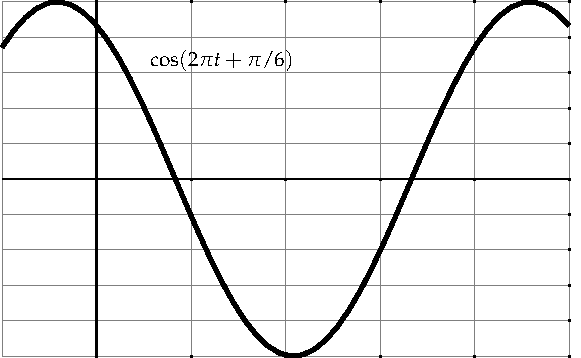
\includegraphics[width=.9\linewidth]{../figs/Sin.pdf}
\end{center}
\end{frame}

\begin{frame}[label={sec:org6535e13}]{Valor medio y valor eficaz}
\begin{itemize}
\item \alert{Valor medio}: $$Y_m=\frac{1}{T}\int_{0}^{T}y(t)$$

\begin{itemize}
\item Para señal sinusoidal:
$$Y_m=\frac{1}{T}\int_{0}^{T}Y_{o}\cdot\cos(\omega\cdot
            t+\phi)\, dt=0$$
\end{itemize}

\item \alert{Valor eficaz}:
$$Y = \sqrt{\frac{1}{T}\cdot\int_{0}^{T}y^{2}(t)}$$

\begin{itemize}
\item Para señal sinusoidal:
\end{itemize}
\end{itemize}

$$Y=\sqrt{\frac{1}{T}\cdot\int_{0}^{T}\left(Y_{o}\cdot\cos(\omega\cdot
      t+\phi)\right)^{2}dt}=\frac{Y_{o}}{\sqrt{2}}$$
\end{frame}

\begin{frame}[label={sec:orgdedbcc4}]{Representación fasorial}
$$\overline{Y}=Y\cdot e^{j\phi}=Y\cdot(\cos(\phi)+\mathrm{j}\cdot\sin(\phi))$$

\begin{center}
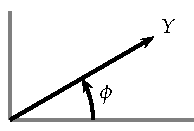
\includegraphics[width=.9\linewidth]{../figs/Fasor.pdf}
\end{center}
\end{frame}

\subsection{Impedancia}
\label{sec:org2add6b5}

\begin{frame}[label={sec:orgd959c53}]{Impedancia}
\end{frame}

\begin{frame}[label={sec:org5019cd3}]{Impedancia}
$$\overline{I}=\frac{\overline{V}}{\overline{Z}}=\frac{V}{Z}\cdot
e^{j(\phi_{V}-\phi_{Z})}=I\cdot e^{j\phi_{I}}$$
\begin{center}
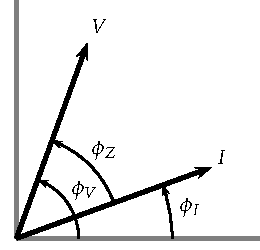
\includegraphics[height=0.4\textheight]{../figs/Impedancia.pdf}
\end{center}
\end{frame}

\begin{frame}[label={sec:org45d234a}]{Convenio de signos para Desfase}
\begin{itemize}
\item La tensión es origen de fases (\(\phi_{V}=0\)).

\item La corriente está retrasada de la tensión un ángulo \(\phi\) positivo:
$$\begin{aligned}
         \phi_{I} & = & -\phi=\phi_{V}-\phi_{Z}\\
         \phi & = & \phi_{z}\\
         i(t) & = & I_{o}\cdot\cos(\omega\cdot t-\phi)
       \end{aligned}$$

\item Por tanto, \alert{si el circuito es inductivo (retrasa fase de corriente
respecto de tensión) \(\phi\) es positivo}.
\end{itemize}
\end{frame}

\begin{frame}[label={sec:orga5e216d}]{Circuito Capacitivo puro}
\begin{center}
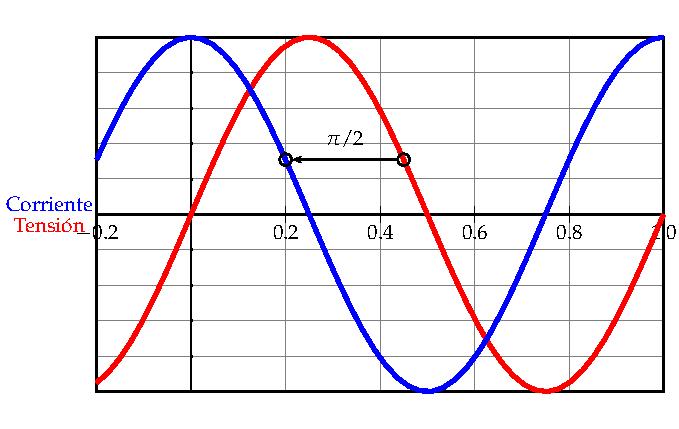
\includegraphics[width=.9\linewidth]{../figs/PlotCircuitoCapacitivoPuro.pdf}
\end{center}
\end{frame}

\begin{frame}[label={sec:org5e9ec77}]{Circuito Inductivo puro}
\begin{center}
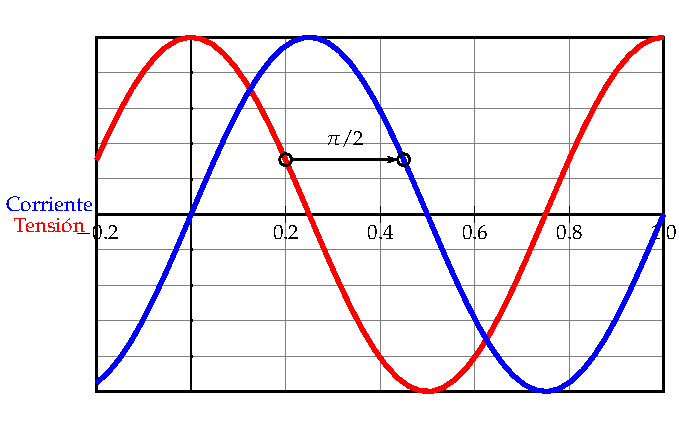
\includegraphics[width=.9\linewidth]{../figs/PlotCircuitoInductivoPuro.pdf}
\end{center}
\end{frame}

\begin{frame}[label={sec:org32798bd}]{Circuito Capacitivo}
\begin{center}
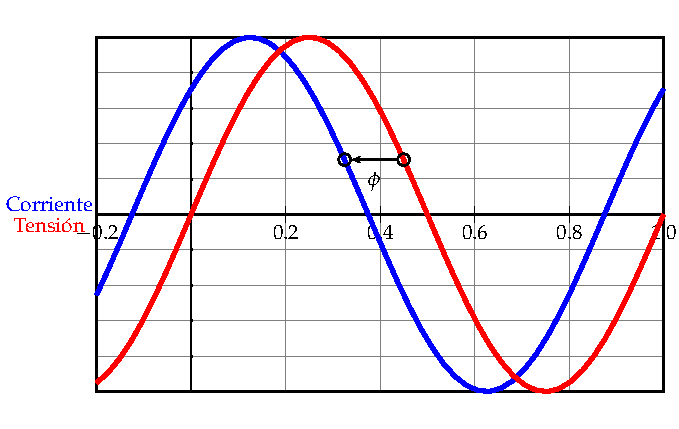
\includegraphics[width=.9\linewidth]{../figs/PlotCircuitoCapacitivo.pdf}
\end{center}
\end{frame}

\begin{frame}[label={sec:org7333f72}]{Circuito Inductivo}
\begin{center}
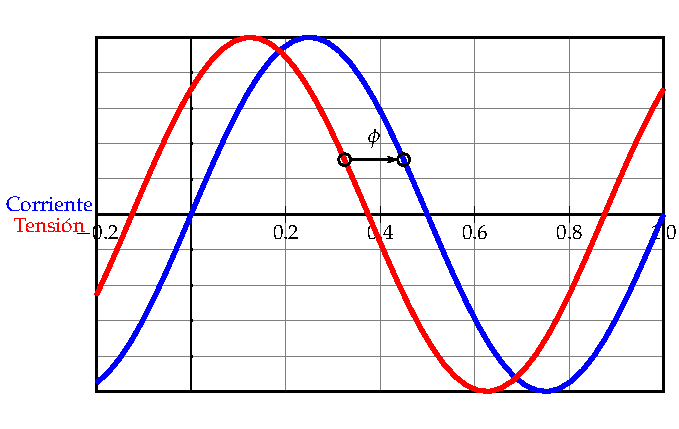
\includegraphics[width=.9\linewidth]{../figs/PlotCircuitoInductivo.pdf}
\end{center}
\end{frame}

\subsection{Potencia}
\label{sec:org3694bb2}

\begin{frame}[label={sec:orgc113b49}]{Circuito Capacitivo puro}
\begin{block}{Potencia}
\begin{center}
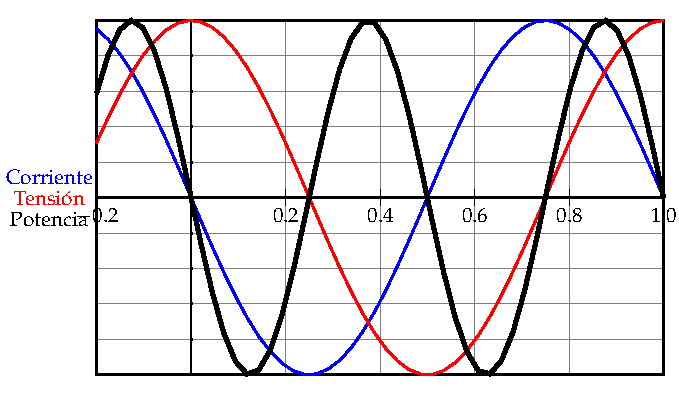
\includegraphics[width=.9\linewidth]{../figs/PlotCircuitoCapacitivoPuro_Potencia.pdf}
\end{center}
\end{block}
\end{frame}

\begin{frame}[label={sec:org5784024}]{Circuito Inductivo puro}
\begin{block}{Potencia}
\begin{center}
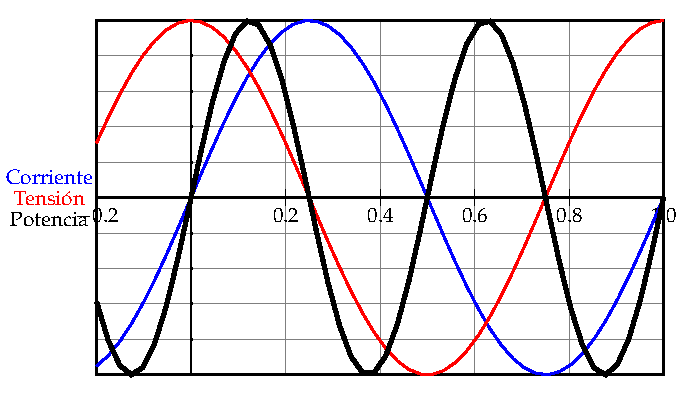
\includegraphics[width=.9\linewidth]{../figs/PlotCircuitoInductivoPuro_Potencia.pdf}
\end{center}
\end{block}
\end{frame}

\begin{frame}[label={sec:org620722f}]{Circuito Capacitivo}
\begin{block}{Potencia}
\begin{center}
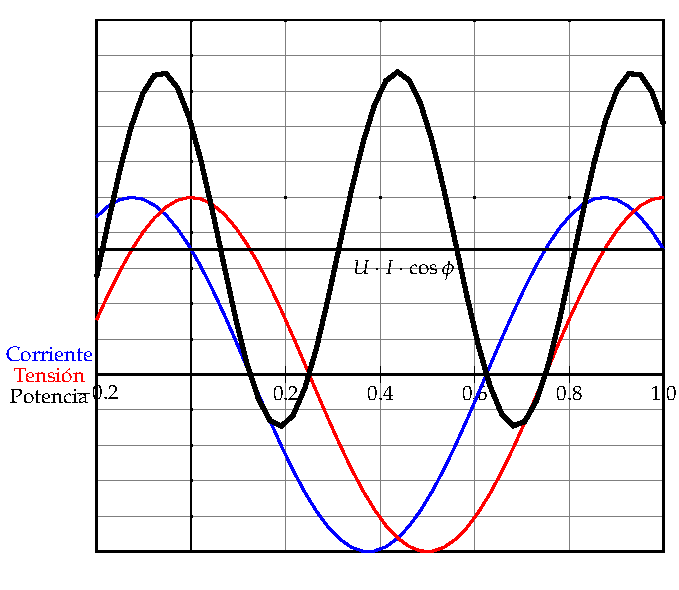
\includegraphics[width=.9\linewidth]{../figs/PlotCircuitoCapacitivo_Potencia.pdf}
\end{center}
\end{block}
\end{frame}

\begin{frame}[label={sec:org4dbd734}]{Circuito Inductivo}
\begin{block}{Potencia}
\begin{center}
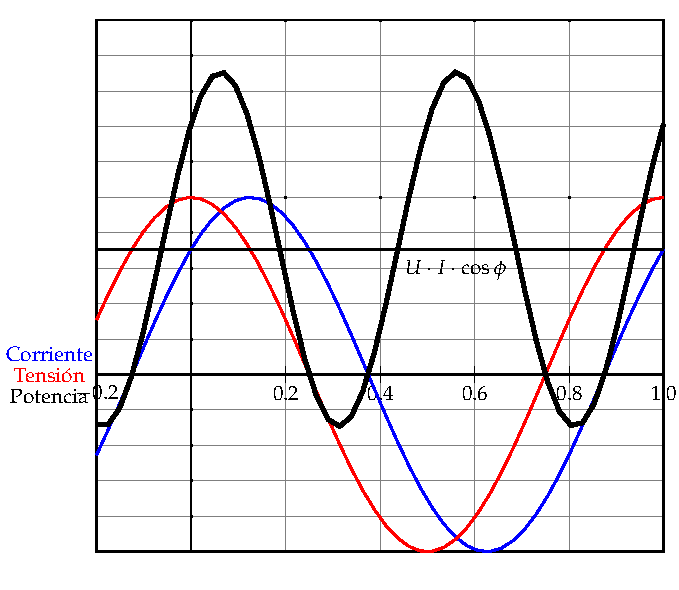
\includegraphics[width=.9\linewidth]{../figs/PlotCircuitoInductivo_Potencia.pdf}
\end{center}
\end{block}
\end{frame}

\begin{frame}[label={sec:org68917ff}]{Potencia Activa, Reactiva y Aparente}
$$\begin{aligned}
  P & = & V\cdot I\cdot\cos(\phi)\\
  Q & = & V\cdot I\cdot\sin(\phi)\\
  S & = & P+jQ\end{aligned}$$
\end{frame}

\begin{frame}[label={sec:orgb725653}]{Potencia de elementos}
\begin{itemize}
\item Una \alert{resistencia sólo consume potencia activa} (\(\cos(\phi)=1\)).

\item Un \alert{condensador no consume potencia activa} (\(\cos(\phi)=0\)), y
\alert{entrega potencia reactiva} (\(\sin(\phi)=-1\))

\item Una \alert{bobina no consume potencia activa} (\(\cos(\phi)=0\)) y \alert{absorbe
potencia reactiva} (\(\sin(\phi)=1\))
\end{itemize}
\end{frame}

\begin{frame}[label={sec:org1ed7caa}]{Teorema de Boucherot}
\end{frame}
\begin{frame}[label={sec:orgf01c219}]{Compensación de reactiva}
\begin{itemize}
\item El factor de potencia (\(\cos(\phi)\)) representa el desfase entre
tensión y corriente.

\item Es la fracción de potencia activa dentro de la potencia aparente.

\item Suponiendo tensión constante, la corriente que debe circular es
\(I=\frac{S}{V}=\frac{P}{V\cdot\cos(\phi)}\).

\item Para alimentar una potencia activa determinada, \alert{la corriente es
tanto más alta cuanto menor el factor de potencia}.

\item \alert{Factores de potencia bajos} obligan a

\begin{itemize}
\item Utilizar \alert{grandes secciones} de cable para transportar la misma
potencia activa

\item Generar \alert{mayor potencia aparente} para alimentar la misma potencia
activa
\end{itemize}
\end{itemize}
\end{frame}

\begin{frame}[label={sec:org25bd798}]{Compensación de reactiva}
\begin{itemize}
\item Comúnmente, el factor de potencia es \alert{inductivo} (máquinas eléctricas
industriales).

\item La red debe suministrar potencia reactiva inductiva (problemas
derivados de bajo factor de potencia)

\item Es necesario alterar localmente el factor de potencia:

\begin{itemize}
\item Solución común: utilizar \alert{bancos de condensadores} como
suministradores de potencia reactiva.
\end{itemize}
\end{itemize}
\end{frame}

\subsection{Trifásica}
\label{sec:org62ed3be}

\begin{frame}[label={sec:org3028e93}]{Motivación de los sistemas trifásicos}
\begin{itemize}
\item La potencia instantánea de un sistema monofásico es pulsante. En un
sistema trifásico la potencia instantánea es constante, evitando
vibraciones y esfuerzos en las máquinas.

\item Para transportar una determinada potencia la masa de conductor
necesaria es un 25\% en un trifásico que en un monofásico.
\end{itemize}
\end{frame}

\begin{frame}[label={sec:org2ef9120}]{Generación de un sistema trifásico}
\begin{center}
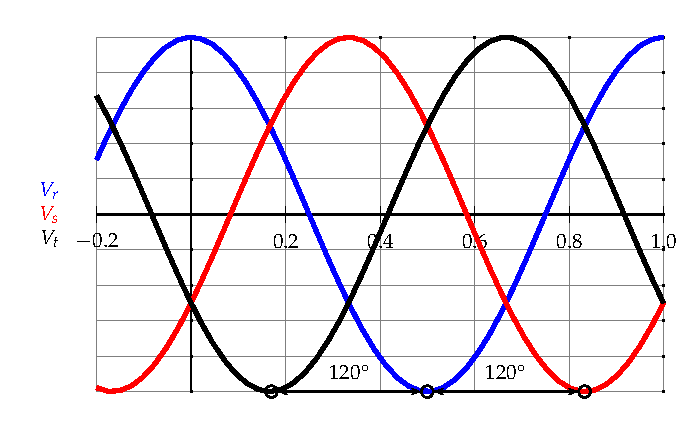
\includegraphics[width=.9\linewidth]{../figs/TensionesTrifasica.pdf}
\end{center}
\end{frame}

\begin{frame}[label={sec:org8547a56}]{Fase y línea}
\begin{block}{Receptor en Estrella (cuatro hilos, 3F+1N)}
$$V_{L}=\sqrt{3}\cdot V_{F}$$ $$I_{F}=I_{L}$$
$$P=3\cdot V_{F}I_{F}\cos(\phi)=\sqrt{3}V_{L}I_{L}\cos(\phi)$$
\begin{center}
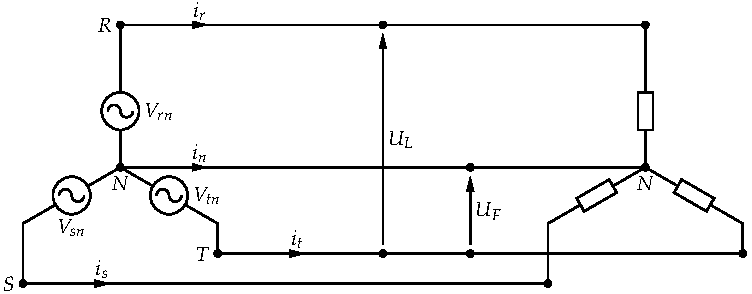
\includegraphics[width=.9\linewidth]{../figs/RedTrifasicaEstrella.pdf}
\end{center}
\end{block}
\end{frame}

\begin{frame}[label={sec:orgbcce042}]{Fase y línea}
\begin{block}{Receptor en Estrella (cuatro hilos, 3F+1N)}
$$V_{L}=\sqrt{3}\cdot V_{F}$$ $$I_{F}=I_{L}$$
$$P=3\cdot V_{F}I_{F}\cos(\phi)=\sqrt{3}V_{L}I_{L}\cos(\phi)$$
\begin{center}
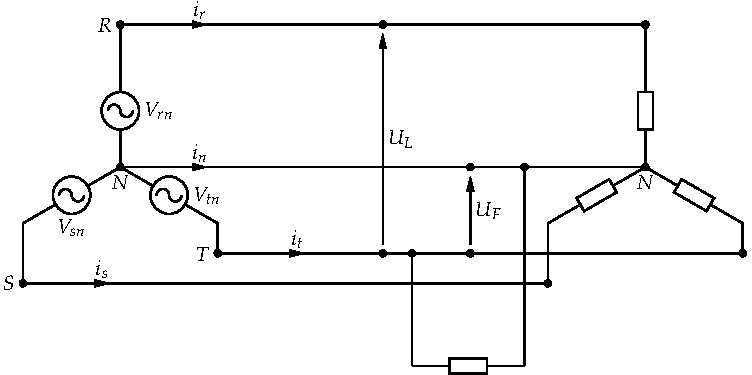
\includegraphics[width=.9\linewidth]{../figs/RedTrifasicaEstrella_CargaMonofasica.pdf}
\end{center}
\end{block}
\end{frame}

\begin{frame}[label={sec:org29ca6c5}]{Fase y línea}
\begin{block}{Receptor en Triangulo (tres hilos, 3F)}
$$V_{L}=V_{F}$$ $$I_{F}=\frac{I_{L}}{\sqrt{3}}$$
$$P=3\cdot V_{F}\cdot I_{F}\cos(\phi)=\sqrt{3}V_{L}I_{L}\cos(\phi)$$
\begin{center}
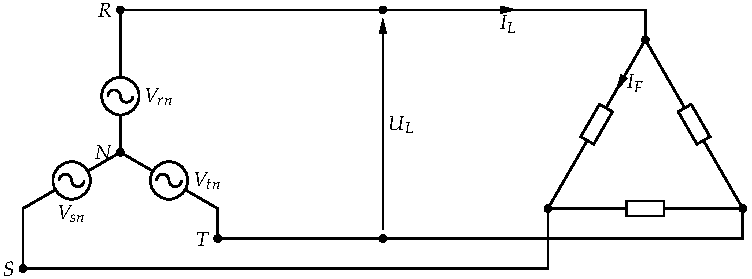
\includegraphics[width=.9\linewidth]{../figs/RedTrifasicaEstrella_CargaTriangulo.pdf}
\end{center}
\end{block}
\end{frame}

\begin{frame}[label={sec:org8c4bb71}]{Fase y línea}
\begin{block}{Receptor en Triangulo (tres hilos, 3F)}
$$V_{L}=V_{F}$$ $$I_{F}=\frac{I_{L}}{\sqrt{3}}$$
$$P=3\cdot V_{F}\cdot I_{F}\cos(\phi)=\sqrt{3}V_{L}I_{L}\cos(\phi)$$
\begin{center}
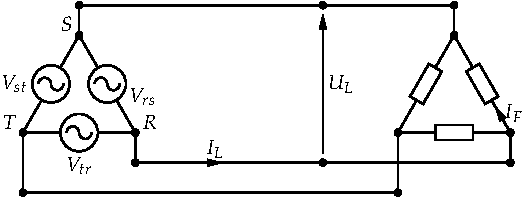
\includegraphics[width=.9\linewidth]{../figs/RedTrifasicaTriangulo.pdf}
\end{center}
\end{block}
\end{frame}

\section{Máquinas Eléctricas}
\label{sec:orgbbb6615}

\subsection{Fundamentos de Electromagnetismo}
\label{sec:org51be9d5}

\begin{frame}[label={sec:org8176e6e}]{Electromagnetismo}
\begin{itemize}
\item Un campo magnético ejerce una fuerza sobre una carga en movimiento.
(Fuerza de Lorentz)
\end{itemize}

\begin{center}
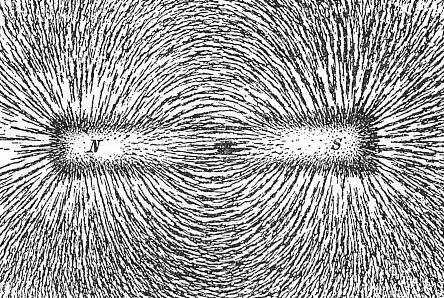
\includegraphics[width=.9\linewidth]{../figs/Magnet0873.png}
\end{center}
\end{frame}

\begin{frame}[label={sec:org98bc87c}]{Electromagnetismo}
\begin{itemize}
\item Una corriente eléctrica crea un campo magnético en torno al
conductor. (Oersted, Biot-Savart)
\end{itemize}

\begin{center}
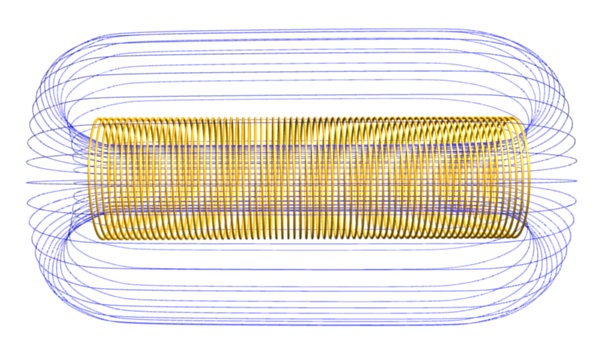
\includegraphics[width=.9\linewidth]{../figs/Solenoide.jpg}
\end{center}
\end{frame}

\begin{frame}[label={sec:org2a262fe}]{Electromagnetismo}
\begin{itemize}
\item Un conductor por el que circula corriente, situado en el seno de un
campo magnético, altera este campo magnético, y experimenta una
fuerza que lo expulsa para disminuir la alteración (Fuerza de Ampere)
\end{itemize}

\begin{center}
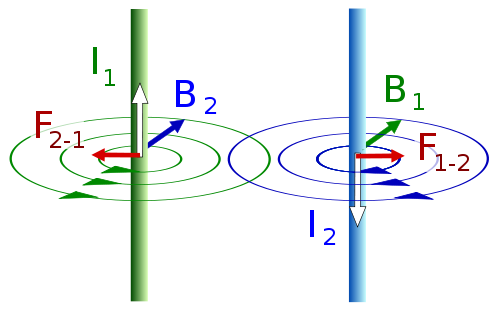
\includegraphics[width=.9\linewidth]{../figs/FuerzasRepulsion.png}
\end{center}

\begin{center}
Vídeo: \href{http://www.youtube.com/watch?v=2j8D\_N1v0tU}{Repulsión entre barras de Alta Tensión}
\end{center}
\end{frame}

\begin{frame}[label={sec:org1b49253}]{Electromagnetismo}
\begin{itemize}
\item Entre los puntos extremos de una espira estática atravesada por un
campo magnético, aparece una \alert{tensión inducida siempre que el flujo
magnético sea variable}. (Ley de Faraday).

\item Esta condición se cumple cuando la \alert{espira está en movimiento,}
cuando el \alert{campo magnético es variable}, o cuando ambas situaciones
coinciden.
\end{itemize}
\end{frame}

\begin{frame}[label={sec:org672ca30}]{Electromagnetismo}
\begin{itemize}
\item La tensión inducida es directamente proporcional a la rapidez con que
cambia en el tiempo el flujo magnético que atraviesa la superficie
encerrada por la espira. $$e=-\frac{\mathrm{d}\phi}{\mathrm{d}t}$$

\item Al elemento que emite el campo magnético se le denomina \alert{inductor} y
aquel que es atravesado por este flujo es el \alert{inducido}.
\end{itemize}
\end{frame}

\begin{frame}[label={sec:orgfaada0f}]{Electromagnetismo}
\begin{center}
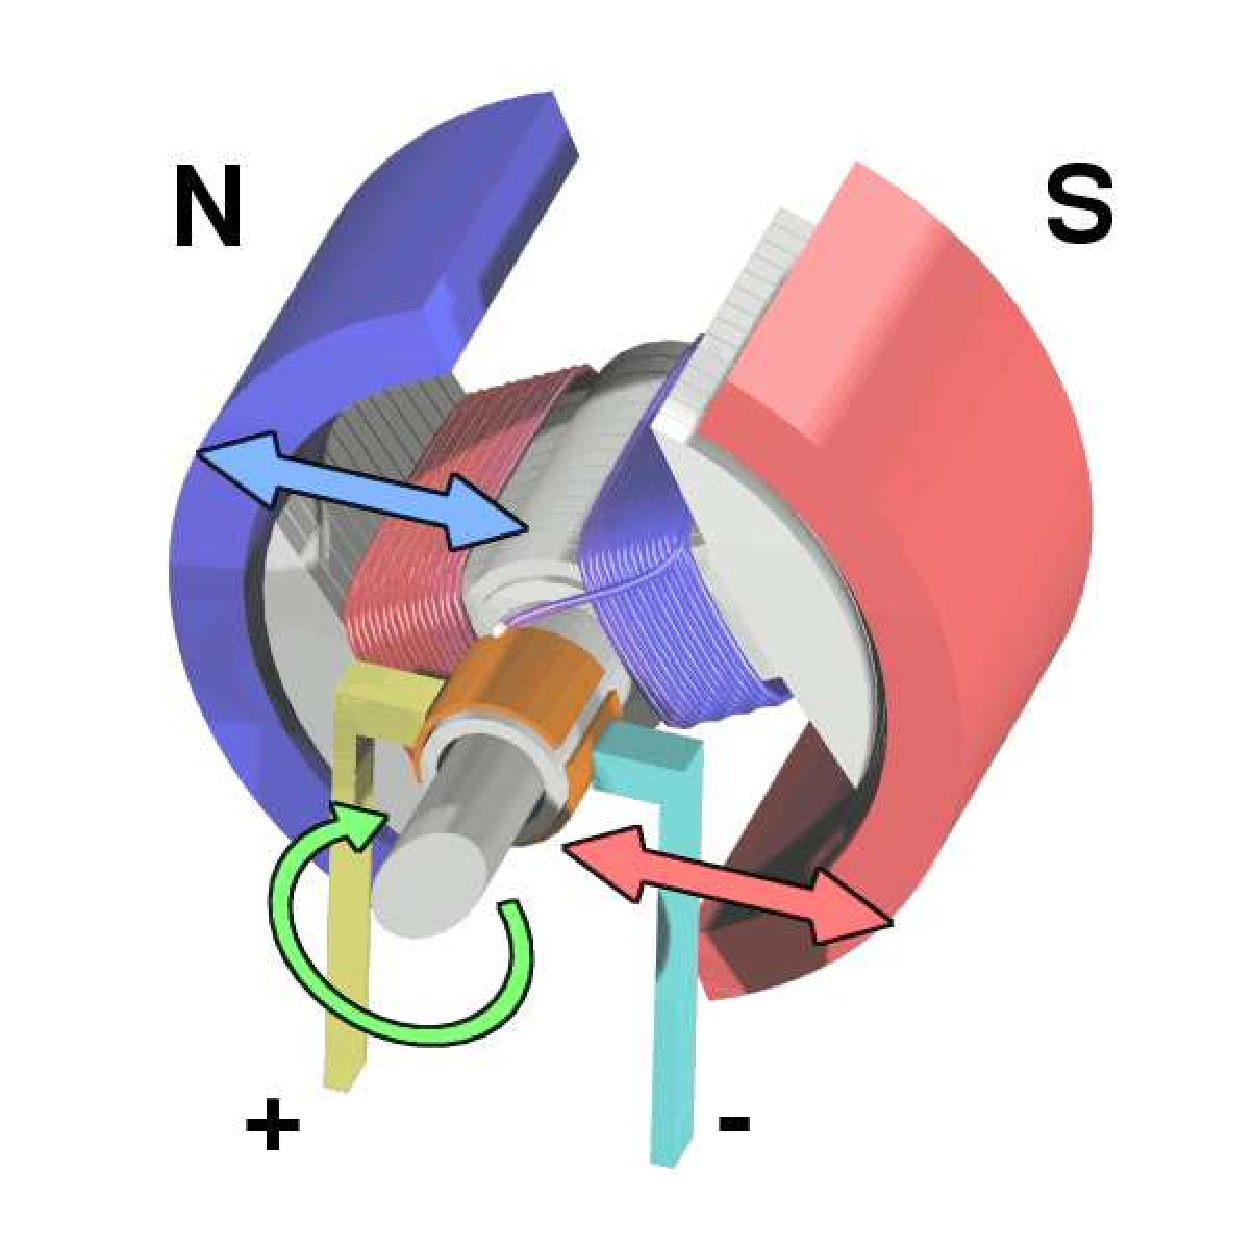
\includegraphics[width=.9\linewidth]{../figs/Electric_motor_cycle_3.pdf}
\end{center}
\end{frame}

\begin{frame}[label={sec:org9dc8615}]{Electromagnetismo}
\begin{block}{Tensión, frecuencia y flujo}
$$\begin{aligned}
  E & = & 4.44\cdot N\cdot\phi\cdot f\end{aligned}$$

\begin{itemize}
\item \(E\) es la tensión inducida; \(N\) número de espiras; \(\phi\) es el flujo
interceptado; \(f\) frecuencia eléctrica

\item El flujo depende proporcionalmente de la tensión e inversamente de la
frecuencia.
\end{itemize}
\end{block}
\end{frame}

\begin{frame}[label={sec:org9b784be}]{Electromagnetismo}
\begin{block}{Par, potencia y velocidad}
$$\begin{aligned}
  P & = & T\cdot\omega\end{aligned}$$

\begin{itemize}
\item \(P\) es potencia mecánica; \(T\) par mecánico; \(\omega\) es la velocidad
angular.

\item El par busca alinear los ejes magnéticos de inductor e inducido, o de
estator y rotor. Una vez que están alineados, el par es nulo.
\end{itemize}
\end{block}
\end{frame}

\subsection{Tipos de máquinas}
\label{sec:org55c59e4}


\begin{frame}[label={sec:orga0ee3a7}]{Relación de Frecuencias}
\begin{block}{Frecuencia eléctrica y velocidad}
$$\begin{aligned}
  f_{2} & = & f_{1}-n\cdot p\end{aligned}$$

\begin{itemize}
\item \(f_{2}\) es la frecuencia en el inducido; \(f_{1}\) es la frecuencia en
el inductor; \(n\) es la velocidad angular; \(p\) es el número de polos.

\item Al utilizar colector de delgas (escobillas) en el inducido, la
frecuencia en el circuito exterior (\(f_{L}\)) es diferente a \(f_{2}\).
\end{itemize}
\end{block}
\end{frame}

\begin{frame}[label={sec:org7cf3bb1}]{Clasificación de máquinas}
\begin{itemize}
\item Estáticas (\(n=0\Rightarrow f_{2}=f_{1}\)): Transformadores

\item Rotativas (\(n\neq0\)):

\begin{itemize}
\item Flujo inductor constante (\(f_{1}=0\Rightarrow f_{2}=n\cdot
            p\))

\begin{itemize}
\item Delgas (\(f_{L}\neq f_{2}\)): Máquinas de corriente continua

\item Anillos (\(f_{L}=f_{2}\)): Máquinas síncronas
\end{itemize}

\item Flujo inductor variable (\(f_{1}>0\Rightarrow
            f_{2}=f_{1}-n\cdot p\))

\begin{itemize}
\item Delgas (\(f_{L}\neq f_{2}\)): Motor universal

\item Anillos (\(f_{L}=f_{2}\)): Máquinas asíncronas
\end{itemize}
\end{itemize}
\end{itemize}
\end{frame}

\begin{frame}[label={sec:org6d01de5}]{Transformador}
\begin{itemize}
\item Un transformador consiste en dos bobinas acopladas magnéticamente.

\item Un transformador ideal tiene las siguientes relaciones entre tensión
y corriente de entrada (primario) y salida (secundario):
\end{itemize}

$$N_{s}\cdot I_{s}=N_{p}\cdot I_{p}$$
$$\frac{V_{p}}{N_{p}}=\frac{V_{s}}{N_{s}}$$

\begin{center}
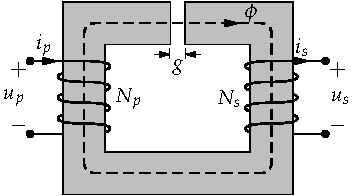
\includegraphics[height=0.3\textheight]{../figs/Transformador2.pdf}
\end{center}
\end{frame}

\begin{frame}[label={sec:orgf08b68b}]{Transformador}
\begin{itemize}
\item Un transformador ideal con relación de transformación \(N_{p}/N_{s}<1\)
(más vueltas en el secundario que en el primario), sube tensión
(\(V_{s}>V_{p}\)) y reduce corriente (\(I_{s}<I_{p}\)).
\end{itemize}

\begin{center}
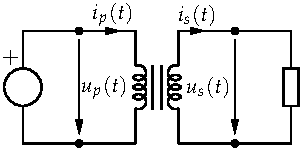
\includegraphics[width=.9\linewidth]{../figs/Transformador.pdf}
\end{center}
\end{frame}

\begin{frame}[label={sec:org43ceaf1}]{Motores}
\begin{block}{Motor DC}
\begin{itemize}
\item \(f_{1}=0\); \(f_{L}=0\);

\item Estator-Inductor alimentado por corriente DC (o imanes permanentes).

\item El colector de delgas transforma la frecuencia de alimentación (DC)
en alterna.

\item Rotor-Inducido gira sincronizado con la frecuencia \guillemotleft{}transformada\guillemotright{}.
\end{itemize}
\end{block}
\end{frame}

\begin{frame}[label={sec:org0d30623}]{Motores}
\begin{block}{Motor asíncrono o de inducción}
\begin{itemize}
\item \(f_{1}\neq0\);

\item Estator-inductor alimentado por una corriente trifásica alterna.
Produce un campo giratorio.

\item Rotor-inducido constituido por espiras cortocircuitadas (jaula de
ardilla).

\item Se produce un par que busca alinear el eje de las espiras con el
campo inducido. El rotor se mueve siguiendo al campo giratorio.

\item La velocidad de giro es inferior a la frecuencia de alimentación
(asíncrono).
\end{itemize}

\begin{center}
Vídeos: Motor de inducción artesanal \href{http://www.youtube.com/watch?v=ZRGlAu0uCHY\&feature=related}{(1)} \href{http://www.youtube.com/watch?v=P-eTLmJC2cQ}{(2)}
\end{center}
\end{block}
\end{frame}
\begin{frame}[label={sec:orgcdfe0c4}]{Generadores}
\begin{block}{Generador Síncrono o Alternador}
\begin{itemize}
\item \(f_{1}=0\);

\item Rotor-inductor alimentado por corriente continua mediante anillos.

\item Estator-inducido constituido por un devanado trifásico.

\item Al aplicar energía mecánica en el eje del rotor y alimentarlo con
corriente continua, se obtiene una fuerza electromotriz en el
estator.

\item Empleado en turbinas hidráulicas y térmicas.
\end{itemize}
\end{block}
\end{frame}

\begin{frame}[label={sec:org8d19ba9}]{Generadores}
\begin{block}{Dinamo}
\begin{itemize}
\item \(f_{1}=0\); \(f_{L}=0\);

\item Estator-Inductor alimentado por corriente DC (o imanes permanentes).

\item El colector de delgas transforma la frecuencia de alimentación (DC)
en alterna.

\item Al aplicar energía mecánica en el eje del rotor y alimentar el
estator con corriente continua, se obtiene una fuerza electromotriz
en el inducido con \(f_{2}\).

\item Las delgas rectifican para obtener \(f_{L}=0\) en la salida.
\end{itemize}
\end{block}
\end{frame}

\section{Aparamenta eléctrica}
\label{sec:orgeb05543}


\subsection{Definición y Funciones}
\label{sec:org062987e}
\begin{frame}[label={sec:org529704d}]{Definición}
\begin{block}{ITC-BT-01}
\begin{description}
\item[{Aparamenta:}] Equipo, aparato o material previsto para ser conectado a un circuito eléctrico con el fin de asegurar una o varias de las siguientes funciones: \alert{protección}, \alert{control}, \alert{seccionamiento}, \alert{conexión}.

\item[{Función de la Aparamenta:}] Garantizar la seguridad de las personas,
la continuidad en el suministro y la protección de los elemento de la
instalación.
\end{description}
\end{block}
\end{frame}

\begin{frame}[label={sec:org5272a08}]{Funciones de la aparamenta}
\begin{itemize}
\item \alert{Protección}:

\begin{itemize}
\item Protección de los elementos de los circuitos contra las tensiones
térmicas y mecánicas de las corrientes de cortocircuito.

\item Protección de las personas en caso de producirse un defecto de
aislamiento.

\item Protección de los dispositivos y aparatos suministrados.
\end{itemize}
\end{itemize}
\end{frame}

\begin{frame}[label={sec:org2724986}]{Funciones de la aparamenta}
\begin{itemize}
\item \alert{Aislamiento}: separar de forma verificable un circuito, un aparato o
un elemento de la planta del resto de un sistema que se encuentra en
tensión, con el fin de que el personal pueda realizar con total
seguridad trabajos en la parte aislada.
\end{itemize}
\end{frame}

\begin{frame}[label={sec:org74ef482}]{Funciones de la aparamenta}
\begin{itemize}
\item \alert{Control:} modificar un sistema cargado en cualquier momento

\begin{itemize}
\item Control funcional (conmutación rutinaria, etc.).

\item Conmutación de emergencia.

\item Operaciones de mantenimiento del sistema de alimentación.
\end{itemize}
\end{itemize}
\end{frame}

\begin{frame}[label={sec:org5958c8b}]{Arco Eléctrico}
\begin{itemize}
\item Descarga eléctrica que se forma entre dos electrodos sometidos a una diferencia de potencial.
\item Durante el tiempo de la descarga se produce una luminosidad muy intensa y un gran desprendimiento de calor.
\item Ambos fenómenos, en caso de ser accidentales, pueden ser sumamente destructivos.
\end{itemize}

\begin{center}
Vídeo: \href{http://www.youtube.com/watch?v=WBTvGqRA4\_0}{Apertura en Alta Tensión}
\end{center}
\end{frame}

\begin{frame}[label={sec:org3e1622d}]{Poder de corte y cierre}
\begin{description}
\item[{Poder de corte:}] intensidad de corriente que este dispositivo es
capaz de cortar, bajo una tensión de restablecimiento determinada.

\item[{Poder de cierre:}] intensidad de corriente que este aparato es capaz
de establecer, bajo una tensión dada.
\end{description}
\end{frame}

\subsection{Tipos de Dispositivos}
\label{sec:orgb0149db}
\begin{frame}[label={sec:org3f4b49a}]{Dispositivos simples}
\begin{block}{Seccionador}
\begin{itemize}
\item Dispositivo de dos posiciones (abierto/cerrado) enclavable y accionado manualmente que proporciona un aislamiento seguro de un circuito cuando está enclavado en la posición abierta.

\item Un seccionador no está diseñado para abrir o cerrar el paso de la corriente.
\end{itemize}
\end{block}

\begin{block}{Interruptor de carga}
\begin{itemize}
\item Dispositivo no automático (accionamiento manual) de dos posiciones (abierto/cerrado).
\item Se utiliza para cerrar y abrir circuitos cargados en condiciones normales de circuitos sin defectos.
\end{itemize}
\end{block}
\end{frame}

\begin{frame}[label={sec:org65d9b81}]{Dispositivos simples}
\begin{block}{Contactor}
\begin{itemize}
\item Dispositivo accionado por solenoide que por lo general se mantiene cerrado mediante una corriente (reducida).

\item Se suelen controlar de forma remota por medio de pulsadores de activación/desactivación.
\end{itemize}
\end{block}

\begin{block}{Fusible}
\begin{itemize}
\item Un filamento o lámina de un metal o aleación de bajo punto de fusión que se intercala en un punto determinado de una instalación eléctrica

\item Se funde por Efecto Joule cuando la intensidad de corriente supere, por un cortocircuito o un exceso de carga.

\item Es capaz de abrir un circuito en carga.
\end{itemize}
\end{block}
\end{frame}

\begin{frame}[label={sec:org5031805}]{Interruptor magnetotérmico}
\begin{itemize}
\item Dispositivo automático capaz de interrumpir la corriente eléctrica de un circuito cuando ésta sobrepasa ciertos valores máximos.

\item El dispositivo consta de dos partes, un electroimán y una lámina bimetálica, conectadas en serie y por las que circula la corriente que va hacia la carga.

\item Su funcionamiento se basa en dos de los efectos producidos por la circulación de corriente eléctrica en un circuito: el magnético y el térmico (efecto Joule).

\item Se emplea para \alert{proteger contra sobreintensidades y sobrecargas}.
\end{itemize}

\begin{center}
Vídeo: \href{http://www.youtube.com/watch?v=c6QqnLgWbCQ}{Apertura de un PIA}
\end{center}
\end{frame}

\begin{frame}[label={sec:orgd2243ee}]{Interruptor Magnetotérmico}
\begin{center}
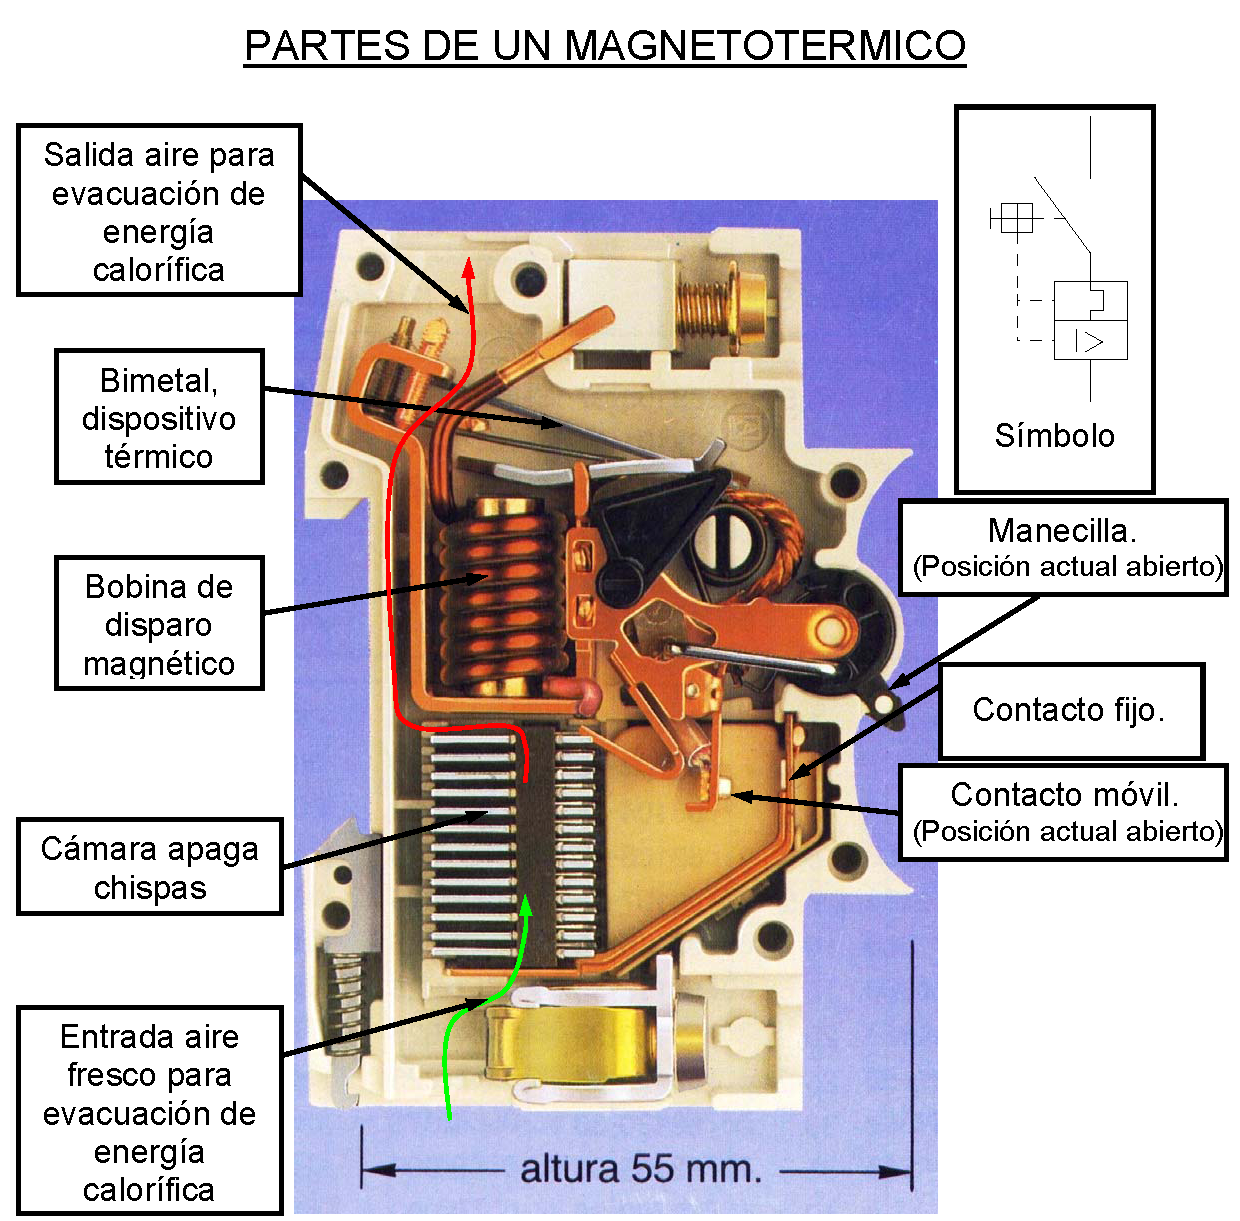
\includegraphics[height=0.8\textheight]{../figs/SeccionMagnetotermico.png}
\end{center}
\end{frame}

\begin{frame}[label={sec:orged100d8}]{Interruptor diferencial}
\begin{itemize}
\item Dispositivo automático capaz de interrumpir la corriente eléctrica de un circuito cuando existe una corriente diferencial residual, indicativa de un defecto de aislamiento.
\item Para la detección emplea un transformador toroidal que abraza a todos los conductores.
\item Cuando existe un defecto, la suma fasorial de las corrientes abarcadas no será nula y, por tanto, aparecerá una intensidad en el secundario del transformador, proporcional al defecto.
\item Se emplea para la \alert{protección de las personas}.
\end{itemize}
\end{frame}

\begin{frame}[label={sec:orgaa617ad}]{Interruptor Diferencial}
\begin{center}
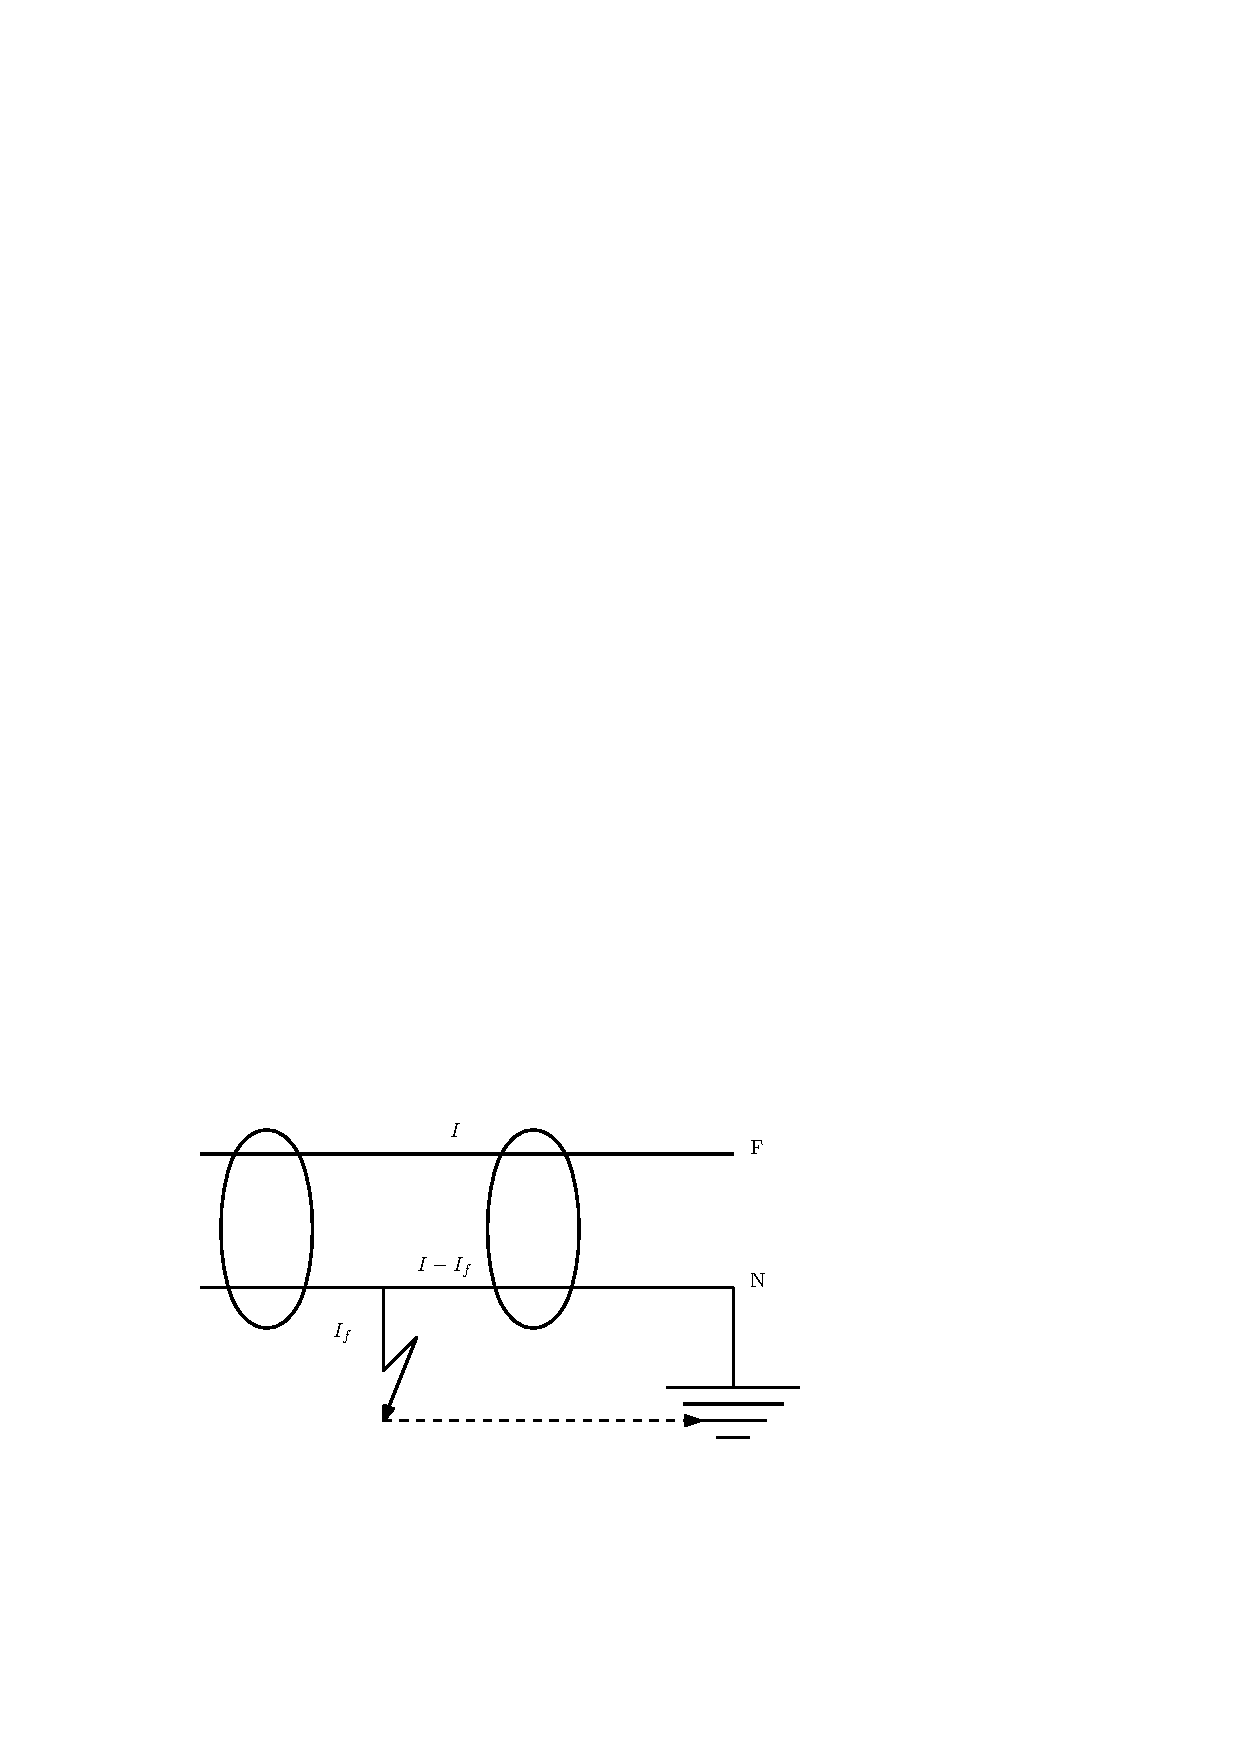
\includegraphics[height=0.3\textheight]{../figs/InterruptorDiferencial.pdf}
\end{center}

\begin{center}
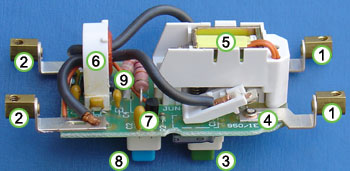
\includegraphics[height=0.3\textheight]{../figs/ResidualCurrentCircuitBreak.jpg}
\end{center}
\end{frame}

\section{Recursos}
\label{sec:org9dd293f}

\begin{frame}[label={sec:org65671ed}]{Bibliografía}
\begin{itemize}
\item \alert{Fraile Mora, J.}: \emph{Circuitos Eléctricos}. Ed. Prentice Hall.

\item \alert{Fraile Mora, J.}: \emph{Máquinas Eléctricas}. Ed. Mc. Graw Hill.

\item \alert{Hayt, W. y Kemmerly, J}: \emph{Análisis de circuitos en ingeniería}. Ed.
Mc. Graw Hill.
\item \alert{C. K. Alexander; M. N. O. Sadiku}, Ed. McGraw-Hill.
\end{itemize}
\end{frame}

\begin{frame}[label={sec:org2c0b3cc}]{Enlaces útiles}
\begin{itemize}
\item \href{http://www.f2i2.net/legislacionseguridadindustrial/Si\_ambito.aspx?id\_am=76}{Reglamento Electrotécnico de Baja Tensión}

\item \href{http://www.schneiderelectric.es/sites/spain/es/productos-servicios/distribucion-electrica/descarga/pdf-guia-diseno-instalaciones-electricas.page}{Guía de diseño de instalaciones eléctricas (Schneider Electric)}

\item \href{http://tuveras.com/index.html}{Tú verás}

\item \href{http://www.directindustry.com/}{Equipos industriales}

\item \href{http://www.preoc.es/}{Base de Precios PREOC}
\end{itemize}
\end{frame}
\end{document}